\documentclass[10pt]{article}
\usepackage{amsmath}
\usepackage{tikz}
\usepackage{enumerate}
\usetikzlibrary{arrows.meta, positioning}

\begin{document}
11/13/2025
\section{Uncertainty Analysis}
When we report an experimental result, we should report:
\\
\begin{center}
$x = \bar{x} \pm U_x$
\\
or
\\
$\mu_x = \bar{x} \pm U_{\bar{x}} $
\end{center}
where, In 95\% of x $
\begin{cases}
U_x = \text{expanded uncertainty of }x
\\
U_{\bar{x}} = \text{expanded uncertainty of }M_x
\end{cases}$
\\
This tolerance term is $U_x$
\\~\\
For measurands that vary continuously, one cannot measure their values exactly, i.e, there will always be
uncertainty
\\~\\



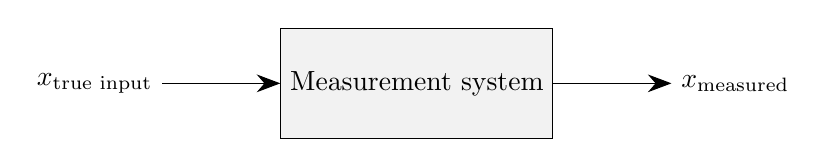
\begin{tikzpicture}[
  block/.style={draw, minimum width=3.2cm, minimum height=1.4cm, fill=gray!10},
  >={Stealth[length=3mm]}
]
% Nodes
\node (u) at (0,0) {$x_{\text{true input}}$};              % input signal
\node[block, right=1.5cm of u] (G) {Measurement system}; % the box
\node[right=1.5cm of G] (y) {$x_{\text{measured}}$};     % output signal

% Arrows
\draw[->] (u) -- (G);   % input to block
\draw[->] (G) -- (y);   % block to output
\end{tikzpicture}
\\~\\
$x_{\text{measured}} = <x> + \alpha_x+\text{Random Errors} + \text{Systematic Errors}$ 
\\~\\
Where,
\begin{itemize}
    \item $<x> = \mu_x=\text{population mean}$
    \item $\alpha_x = fluctuation$
    \item Random Error - Intrinsic to the measurement sytem itelf(ex. noise)
    \begin{itemize}
        \item Generally different for each successuve measurement
    \end{itemize}
    \item Systematic error (symbol $\beta$) - Occurs in the same way each time a measurement is made (ex. A thermometer always reads 1 $C^{\circ}$ too high)
    \item Elemental error
    \begin{itemize}
        \item An identifiable error source
        \item Classifies as either random or SystematicAlso arise from environent variation
    \end{itemize}
\end{itemize}

\begin{center}
    Examples:
\\
\begin{tabular}{|c|c|c|}
    \hline
    accuracy & systematic & $\beta$
    \\
    \hline
    hysterisis & systematic & $\beta$
    \\
    \hline
    installation & systematic & $\beta$
    \\
    \hline
    linearity & systematic & $\beta$
    \\
    \hline
    repeatability & systematic & $\beta$
    \\
    \hline
    noise & random & $\epsilon$
    \\
    \hline
    environmental & random & $\epsilon$
    \\
    \hline
    resolution & random & $\epsilon$
    \\
    \hline
    digitization & systematic & $\beta$
    \\
    \hline
    reading & random & $\epsilon$
    \\
    \hline
    .&.&.
    \\
    \hline
    .&.&.
    \\
    \hline
    .&.&.
    \\
    \hline
\end{tabular}
\end{center}

\end{document}